% This file was created by matlab2tikz.
%
%The latest updates can be retrieved from
%  http://www.mathworks.com/matlabcentral/fileexchange/22022-matlab2tikz-matlab2tikz
%where you can also make suggestions and rate matlab2tikz.
%



% Define custom colors
\definecolor{mycolor1}{rgb}{0.00000,0.44700,0.74100}%
\definecolor{mycolor2}{rgb}{0.85000,0.32500,0.09800}%
\definecolor{mycolor3}{rgb}{0.92900,0.69400,0.12500}%
\definecolor{mycolor4}{rgb}{0.49400,0.18400,0.55600}%




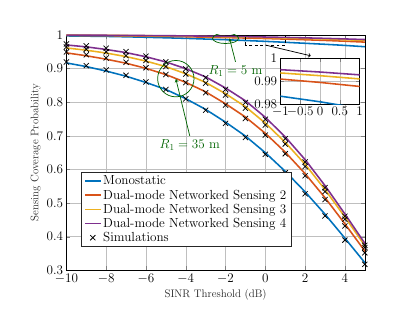
\begin{tikzpicture}[scale=0.33, transform shape,font=\Large]

% Main plot
\begin{axis}[%
width=4.521in,
height=3.566in,
at={(0.758in,0.481in)},
scale only axis,
xmin=-10,
xmax=5,
xlabel style={font=\large\color{white!15!black}},
xlabel={SINR Threshold (dB)},
ylabel style={font=\large\color{white!15!black}},
ylabel={Sensing Coverage Probability},
ymin=0.3,
ymax=1,
axis background/.style={fill=white},
xmajorgrids,
ymajorgrids,
legend style={at={(0.05,0.1)}, anchor=south west, legend cell align=left, align=left, draw=white!15!black}
]

% R1 = 5 plots
\addplot [line width=0.6mm, color=mycolor1] table[row sep=crcr]{%
-10 0.99706\\ -9 0.99638\\ -8 0.99564\\ -7 0.99448\\ -6 0.99308\\ -5 0.9915\\ -4 0.98988\\ -3 0.98778\\ -2 0.98594\\ -1 0.9834\\ 0 0.98098\\ 1 0.97814\\ 2 0.97518\\ 3 0.97222\\ 4 0.96892\\ 5 0.965\\ 6 0.96098\\ 7 0.95676\\ 8 0.9523\\ 9 0.94752\\ 10 0.94226\\};
\addlegendentry{Monostatic}

\addplot [line width=0.6mm, color=mycolor2] table[row sep=crcr]{%
-10 0.9986\\ -9 0.99838\\ -8 0.99798\\ -7 0.99732\\ -6 0.99654\\ -5 0.99574\\ -4 0.99472\\ -3 0.99336\\ -2 0.99224\\ -1 0.99082\\ 0 0.98936\\ 1 0.98762\\ 2 0.9857\\ 3 0.98372\\ 4 0.98134\\ 5 0.97872\\ 6 0.97598\\ 7 0.97296\\ 8 0.97008\\ 9 0.96656\\ 10 0.96242\\};
\addlegendentry{Dual-mode Networked Sensing 2}

\addplot [line width=0.6mm, color=mycolor3] table[row sep=crcr]{%
-10 0.99912\\ -9 0.99896\\ -8 0.99876\\ -7 0.99834\\ -6 0.99774\\ -5 0.99714\\ -4 0.9963\\ -3 0.99538\\ -2 0.99456\\ -1 0.99346\\ 0 0.99228\\ 1 0.99088\\ 2 0.9895\\ 3 0.98782\\ 4 0.9857\\ 5 0.98362\\ 6 0.98144\\ 7 0.97926\\ 8 0.97694\\ 9 0.97408\\ 10 0.97042\\};
\addlegendentry{Dual-mode Networked Sensing 3}

\addplot [line width=0.6mm, color=mycolor4] table[row sep=crcr]{%
-10 0.99932\\ -9 0.99918\\ -8 0.99904\\ -7 0.9987\\ -6 0.99826\\ -5 0.99784\\ -4 0.99726\\ -3 0.99652\\ -2 0.99578\\ -1 0.99488\\ 0 0.99386\\ 1 0.99264\\ 2 0.99134\\ 3 0.98992\\ 4 0.98818\\ 5 0.98636\\ 6 0.98456\\ 7 0.98276\\ 8 0.98068\\ 9 0.97796\\ 10 0.97456\\};
\addlegendentry{Dual-mode Networked Sensing 4}


\addplot [color=white, draw=none, mark=x, thick, mark size=4pt, mark options={ black}]
  table[row sep=crcr]{%
-10	0.919558676028084\\
-9	0.908757147156184\\
-8	0.896074691296055\\
-7	0.879919759277834\\
-6	0.86029455966336\\
-5	0.838031409422827\\
-4	0.809751223898491\\
-3	0.776151545363908\\
-2	0.737014925373134\\
-1	0.695079033701163\\
0	0.644942928039702\\
1	0.590033750248164\\
2	0.52757665677547\\
3	0.461635842152112\\
4	0.389866929521932\\
5	0.317849758787043\\
};
\addlegendentry{Simulations}


\addplot [color=white, draw=none, mark=x, thick, mark size=4pt, mark options={ black}]
  table[row sep=crcr]{%
-10	0.949468405215647\\
-9	0.94103721536764\\
-8	0.931492822005823\\
-7	0.918655967903711\\
-6	0.902354473499649\\
-5	0.882404721416425\\
-4	0.858187631131981\\
-3	0.82827517447657\\
-2	0.791283582089552\\
-1	0.751406700467243\\
0	0.702133995037221\\
1	0.646615048640063\\
2	0.581048466864491\\
3	0.510374839283948\\
4	0.43181862986693\\
5	0.352033080634045\\
6	0.27323971324757\\
7	0.199097242665097\\
8	0.135008801095247\\
9	0.0851357928550569\\
10	0.0465179437439379\\
};



\addplot [color=white, draw=none, mark=x, thick, mark size=4pt, mark options={ black}]
  table[row sep=crcr]{%
-10	0.9641925777332\\
-9	0.957648711004113\\
-8	0.94984439313322\\
-7	0.938455366098295\\
-6	0.924055705841098\\
-5	0.906011803541062\\
-4	0.883784593865521\\
-3	0.856131605184447\\
-2	0.821034825870647\\
-1	0.781986280942439\\
0	0.732248138957816\\
1	0.67564026206075\\
2	0.608565776458951\\
3	0.534150924735437\\
4	0.45200591424347\\
5	0.367726690952053\\
6	0.284533045271531\\
7	0.206221175547051\\
8	0.139409348718952\\
9	0.0872773289204711\\
10	0.0475848690591659\\
};


\addplot [color=white, draw=none, mark=x, thick, mark size=4pt, mark options={ black}]
  table[row sep=crcr]{%
-10	0.973119358074223\\
-9	0.967559434246163\\
-8	0.960546129906636\\
-7	0.950351053159478\\
-6	0.936900110209398\\
-5	0.91999599879964\\
-4	0.89897092616645\\
-3	0.872502492522433\\
-2	0.838009950248756\\
-1	0.799463167312854\\
0	0.74941935483871\\
1	0.691522731784793\\
2	0.622373887240356\\
3	0.545781821778261\\
4	0.460877279448004\\
5	0.374401890321945\\
6	0.288637925955023\\
7	0.208595819841036\\
8	0.140641502053589\\
9	0.0879003212304098\\
10	0.0478176527643065\\
};


% R1 = 35 plots
\addplot [line width=0.6mm, color=mycolor1] table[row sep=crcr]{%
-10 0.9168\\ -9 0.90594\\ -8 0.89258\\ -7 0.87728\\ -6 0.85866\\ -5 0.83778\\ -4 0.81048\\ -3 0.77848\\ -2 0.7407\\ -1 0.69918\\ 0 0.64978\\ 1 0.5944\\ 2 0.53338\\ 3 0.46676\\ 4 0.39552\\ 5 0.32284\\ 6 0.25172\\ 7 0.18484\\ 8 0.12672\\ 9 0.08074\\ 10 0.04488\\};


\addplot [line width=0.6mm, color=mycolor2] table[row sep=crcr]{%
-10 0.94662\\ -9 0.93812\\ -8 0.92786\\ -7 0.9159\\ -6 0.90064\\ -5 0.88214\\ -4 0.85896\\ -3 0.83076\\ -2 0.79524\\ -1 0.75584\\ 0 0.7074\\ 1 0.6514\\ 2 0.58744\\ 3 0.51604\\ 4 0.43808\\ 5 0.35756\\ 6 0.27824\\ 7 0.2029\\ 8 0.13806\\ 9 0.08746\\ 10 0.04796\\};


\addplot [line width=0.6mm, color=mycolor3] table[row sep=crcr]{%
-10 0.9613\\ -9 0.95468\\ -8 0.94614\\ -7 0.93564\\ -6 0.9223\\ -5 0.90574\\ -4 0.88458\\ -3 0.8587\\ -2 0.82514\\ -1 0.7866\\ 0 0.73774\\ 1 0.68064\\ 2 0.61526\\ 3 0.54008\\ 4 0.45856\\ 5 0.3735\\ 6 0.28974\\ 7 0.21016\\ 8 0.14256\\ 9 0.08966\\ 10 0.04906\\};


\addplot [line width=0.6mm, color=mycolor4] table[row sep=crcr]{%
-10 0.9702\\ -9 0.96456\\ -8 0.9568\\ -7 0.9475\\ -6 0.93512\\ -5 0.91972\\ -4 0.89978\\ -3 0.87512\\ -2 0.8422\\ -1 0.80418\\ 0 0.75504\\ 1 0.69664\\ 2 0.62922\\ 3 0.55184\\ 4 0.46756\\ 5 0.38028\\ 6 0.29392\\ 7 0.21258\\ 8 0.14382\\ 9 0.0903\\ 10 0.0493\\};











\definecolor{darkgreen}{rgb}{0.00000,0.39200,0.00000} % Define dark green

\draw [stealth-,thick, darkgreen] (axis cs:-1.8,0.99) -- (axis cs:-1.5,0.92) node[below]{$R_1=5$ m};
\draw [thick, darkgreen] (-2,0.99) ellipse (0.5cm and 0.2cm); % Ellipse position unchanged

\draw [stealth-,thick, darkgreen] (axis cs:-4.5,0.87) -- (axis cs:-3.8,0.7) node[below]{$R_1=35$ m}; % Arrow adjusted
\draw [thick, darkgreen] (-4.5,0.87) ellipse (0.7cm and 0.7cm); % Ellipse adjusted








% Highlight zoom region
\draw [dashed, thick] (axis cs:-1,0.97) rectangle (axis cs:1,1);

% Arrow from the middle of the bottom side of the zoom region to above the inset
\draw[->, thick] (axis cs:0,0.97) -- (3.7in,4.55in);

\end{axis}

% Zoom-in inset
\begin{axis}[%
width=1.2in,
height=0.7in,
at={(4in,3in)}, % Position inset plot
scale only axis,
xmin=-1,
xmax=1,
ymin=0.98,
ymax=1,
ytick={0.98, 0.99, 1}, % Specify y-axis tick values
axis background/.style={fill=white},
xmajorgrids,
ymajorgrids
]



% Zoomed-in plots (only R1 = 5)
\addplot [line width=0.6mm, color=mycolor1] table[row sep=crcr]{-1 0.9834\\ 0 0.98098\\ 1 0.97814\\};
\addplot [line width=0.6mm, color=mycolor2] table[row sep=crcr]{-1 0.99082\\ 0 0.98936\\ 1 0.98762\\};
\addplot [line width=0.6mm, color=mycolor3] table[row sep=crcr]{-1 0.99346\\ 0 0.99228\\ 1 0.99088\\};
\addplot [line width=0.6mm, color=mycolor4] table[row sep=crcr]{-1 0.99488\\ 0 0.99386\\ 1 0.99264\\};



\end{axis}

\end{tikzpicture}


